\documentclass[tikz,border=6pt]{standalone}
\usepackage{xcolor}
\usetikzlibrary{arrows.meta,decorations.pathmorphing,calc,positioning,fit,backgrounds,shapes.geometric}
\definecolor{red}{HTML}{A50F2D}\definecolor{ink}{HTML}{141414}\definecolor{gry}{HTML}{5F5F5F}\definecolor{lgry}{HTML}{E6E6E6}
\definecolor{blu}{HTML}{2B6CB0}\definecolor{teal}{HTML}{1B9E8F}\definecolor{org}{HTML}{E8702A}\definecolor{grn}{HTML}{2E9E5B}\definecolor{mag}{HTML}{D81B60}\definecolor{pur}{HTML}{5B2C83}
\tikzset{fibre/.style={ink,line width=1.6pt,line cap=round},
 sis1/.style={org,line width=1.8pt,line cap=round},sis2/.style={blu,line width=1.8pt,line cap=round},
 lab/.style={font=\sffamily\small,text=ink},lbl/.style={font=\sffamily\footnotesize,text=gry,align=center},ttl/.style={font=\sffamily\bfseries\small,text=ink},
 ctcf/.style={-{Triangle[length=5pt,width=6pt]},pur,line width=2.4pt},
 cohesin/.style={grn,line width=1.6pt}}

% ---- shared drawing macros: a DNA duplex is a dark tube with a light core
\newcommand{\dx}[2][ink]{\draw[line width=3.6pt,#1,line cap=round] #2; \draw[line width=1.3pt,white,line cap=round] #2;}
% omega-shaped loop: base at (x,y), radius r
\newcommand{\omegapath}[3]{(#1-0.35,#2) .. controls (#1-0.35,#2+0.45) and (#1-#3,#2+0.35) .. (#1-#3,#2+#3+0.45) arc[start angle=180,end angle=0,radius=#3] .. controls (#1+#3,#2+0.35) and (#1+0.35,#2+0.45) .. (#1+0.35,#2)}
% replication eye: origin at (x,y), half width w, half height h
\newcommand{\eyetop}[4]{(#1-#3,#2) .. controls (#1-#3*0.5,#2+#4*1.33) and (#1+#3*0.5,#2+#4*1.33) .. (#1+#3,#2)}
\newcommand{\eyebot}[4]{(#1-#3,#2) .. controls (#1-#3*0.5,#2-#4*1.33) and (#1+#3*0.5,#2-#4*1.33) .. (#1+#3,#2)}
\newcommand{\eye}[4]{\dx[org]{\eyetop{#1}{#2}{#3}{#4}}\dx[blu]{\eyebot{#1}{#2}{#3}{#4}}\fill[teal] (#1-#3,#2) circle (3.2pt) (#1+#3,#2) circle (3.2pt);}
\newcommand{\ring}[3]{\draw[grn,line width=1.8pt] (#1,#2) ellipse (#3 and #3*1.35);}
\newcommand{\gseg}[3]{\dx[gry]{(#2,#1) -- (#3,#1)}}

\begin{document}
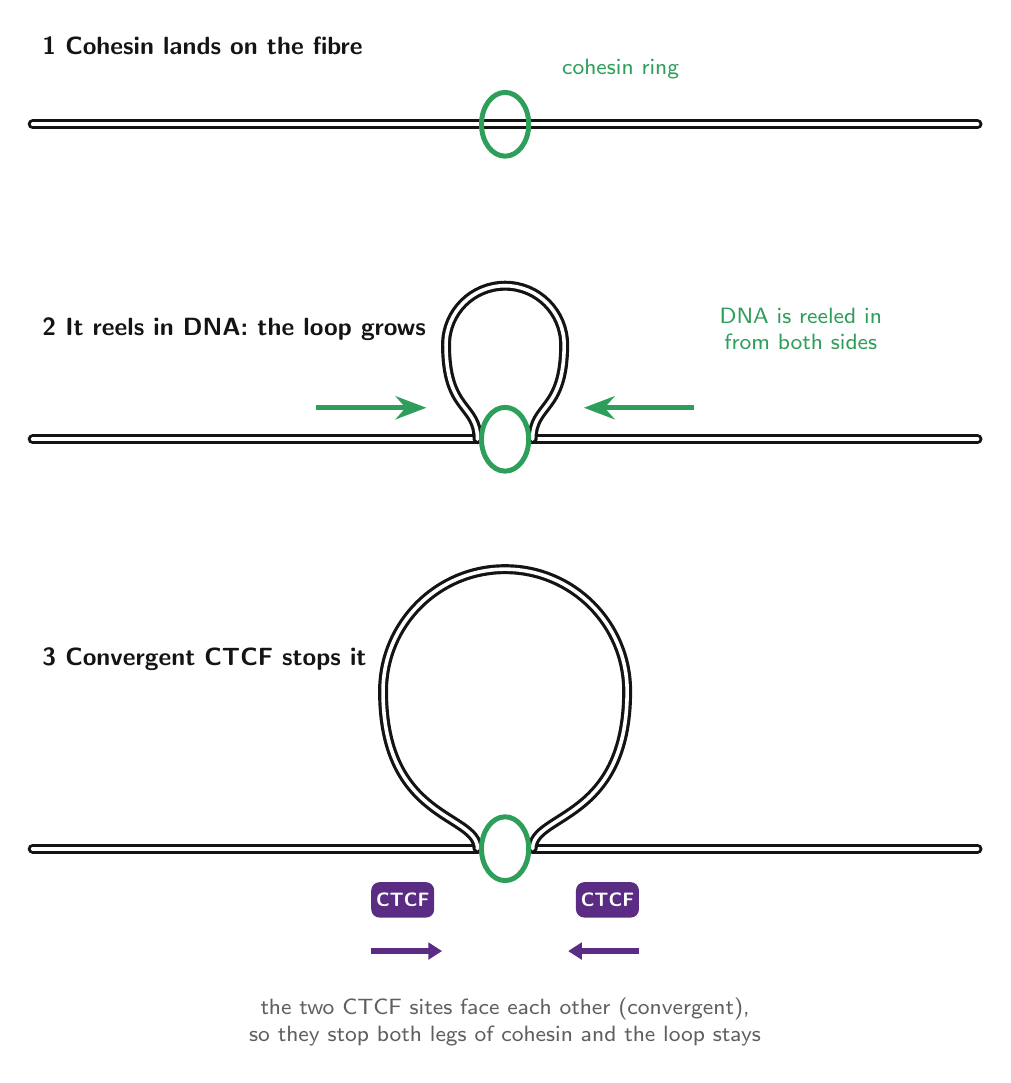
\begin{tikzpicture}[font=\sffamily\small,>=Stealth]
\node[ttl,anchor=west] at (0,1.0) {1  Cohesin lands on the fibre};
\node[ttl,anchor=west] at (0,-2.6) {2  It reels in DNA: the loop grows};
\node[ttl,anchor=west] at (0,-6.8) {3  Convergent CTCF stops it};
% 1
\dx{(0,0) -- (12,0)} \ring{6}{0}{0.3} \node[lbl,grn,anchor=west] at (6.6,0.7) {cohesin ring};
% 2
\dx{(0,-4) -- (5.65,-4)} \dx{(6.35,-4) -- (12,-4)} \dx{\omegapath{6}{-4}{0.75}} \ring{6}{-4}{0.3}
\draw[->,grn,line width=1.8pt] (3.6,-3.6) -- (5.0,-3.6); \draw[->,grn,line width=1.8pt] (8.4,-3.6) -- (7.0,-3.6);
\node[lbl,grn,align=center,anchor=west] at (8.6,-2.6) {DNA is reeled in\\ from both sides};
% 3
\dx{(0,-9.2) -- (5.65,-9.2)} \dx{(6.35,-9.2) -- (12,-9.2)} \dx{\omegapath{6}{-9.2}{1.55}} \ring{6}{-9.2}{0.3}
\foreach \x/\d in {4.7/1,7.3/-1}{
  \node[fill=pur,rounded corners=3pt,minimum width=0.8cm,minimum height=0.45cm,text=white,font=\sffamily\bfseries\scriptsize,inner sep=1pt] at (\x,-9.85) {CTCF};
  \draw[ctcf] (\x-0.4*\d,-10.5) -- (\x+0.5*\d,-10.5);}
\node[lbl] at (6,-11.4) {the two CTCF sites face each other (convergent),\\ so they stop both legs of cohesin and the loop stays};
\end{tikzpicture}
\end{document}
